\documentclass{article}

% if you need to pass options to natbib, use, e.g.:
% \PassOptionsToPackage{numbers, compress}{natbib}
% before loading nips_2016
%
% to avoid loading the natbib package, add option nonatbib:
% \usepackage[nonatbib]{nips_2016}

\PassOptionsToPackage{numbers,sort&compress}{natbib}
\usepackage[final]{nips_2016} % produce camera-ready copy

\usepackage[utf8]{inputenc} % allow utf-8 input
\usepackage[T1]{fontenc}    % use 8-bit T1 fonts
\usepackage{hyperref}       % hyperlinks
\usepackage{url}            % simple URL typesetting
\usepackage{booktabs}       % professional-quality tables
\usepackage{amsfonts}       % blackboard math symbols
\usepackage{nicefrac}       % compact symbols for 1/2, etc.
\usepackage{microtype}      % microtypography
\usepackage{xcolor}         % color text
\usepackage{subcaption}
\usepackage{enumitem}
\usepackage{subcaption}
\usepackage{booktabs}
\usepackage{titlesec}
\usepackage{svg}
\usepackage{graphicx}
\usepackage{float}
\setlist{nosep}

\titlespacing*{\subsection}
  {0pt}{0.3ex}{0.1ex}

\title{Predicting Long-Term Chart Success through Multi-Cluster Music Representations}

% The \author macro works with any number of authors. There are two
% commands used to separate the names and addresses of multiple
% authors: \And and \AND.
%
% Using \And between authors leaves it to LaTeX to determine where to
% break the lines. Using \AND forces a line break at that point. So,
% if LaTeX puts 3 of 4 authors names on the first line, and the last
% on the second line, try using \AND instead of \And before the third
% author name.

\author{
  S2876894\\
  %% examples of more authors
  \And
  S2844528\\
 \And
  S2843292\\
  \And
  S2821285\\
}

\begin{document}

\maketitle

\begin{abstract}
% This project predicts sustained Spotify chart success which is defined as prevailing in the Top 200 for at least eight consecutive weeks on global and regional data from 2017 to 2023. For the representation of songs, we create a multi-dimensional embedding using independent clustering schemes, which model different facets of success: audio characteristics, artist reputation, collaboration networks, and market reach. These cluster memberships serve as interpretable meta-features for downstream classification models, with which we forecast long-term viability by effectively reducing the feature complexity.
This study predicts sustained Spotify chart success using global and regional data spanning 2017–2023. Songs are represented via multi-dimensional embeddings derived from independent clustering schemes that capture audio features, artist reputation, collaboration networks, and market reach. Leveraging these cluster-based meta-features, downstream classifiers and regressors are trained to predict long-term chart viability while reducing feature complexity. The best binary classifier achieved 0.690 ROC-AUC; multiclass F1-score reached 58.9\%. Regression of chart duration attained RMSE of 5.35 weeks ($R^2$ =0.716). Ablation confirmed the proposed meta-feature approach yields significant predictive gains over raw audio features alone, confirming its interpretability and effectiveness. 
\end{abstract}
\vspace{-1em}

\section{Introduction}
\vspace{-0.6em}
\subsection{Background and Motivation}
The music industry has undergone a radical transformation in modern times, due to the rise of digital streaming platforms, which generate an enormous amount of consumption data on a daily basis. Accordingly, understanding and predicting what makes certain songs achieve enduring popularity has become an issue of growing academic and commercial interest. Predictive modeling of a song's success can help record labels, producers, and recommendation systems make strategic decisions on talent discovery, release planning, and marketing optimization.\\
Although previous works in this area of hit song prediction have utilized machine learning models on raw audio or popularity features \cite{gulmatico2022spotipred, martin2020multimodal} these approaches often struggle to generalize across contexts, or provide
interpretable insights into why certain songs succeed. Music is inherently multi-dimensional;
this involves not only sonic characteristics but also temporal trends, artist networks, and geographic influence;
and performance dynamics. Capturing these varied influences in a single framework calls for a
more overarching approach than the traditional feature-based models.
\subsection{Objective and Research Problem}
The objective of the project is to develop a predictive framework that determines whether newly
released tracks will reach continued chart success, defined as remaining in Spotify's Top 200
for at least eight consecutive weeks. In order to achieve this, the project develops a multi-dimensional representation of each song through independent clustering across seven conceptual dimensions. 
Each cluster captures latent relationships in a particular domain, delivering interpretable groupings such as “High-Energy Dance”, “Rising Star”, or “Slow Burn Success”. The resulting cluster memberships
are then combined as meta-features for classification and regression models that predict multiple interpretations of long-term chart retention.

% \textcolor{red}{Can remove if it takes up too much space.}
% \begin{itemize}
%     \item Audio and Musical Style
%     \item Artist Success Tier
%     \item Temporal and Release Patterns
%     \item Collaboration Network Position
%     \item Geographic Market Appeal
%     \item Chart Performance Patterns
%     \item Audio Evolution and Innovation
% \end{itemize}


\subsection{Significance and Contribution}
This project introduces a multi-cluster meta-feature framework for music success prediction, designed to enhance interpretability and reduce feature dimensionality. Instead of directly feeding 15+ raw continuous features into a model, the approach converts them into 5-7 categorical cluster assignments, allowing the model to learn relationships between interpretable song “archetypes” and chart success outcomes. 
% Such representations can uncover cross-dimensional dependencies, such as whether “Rising Stars” in “High-Energy Dance” clusters perform better than “Established Artists” in “Mellow Acoustic” clusters offering richer analytical insight than raw feature correlations.

From a methodological standpoint, this strategy also supports \textbf{non-linear interactions} between musical, social, and temporal factors, which linear models may otherwise fail to capture. Beyond predictive performance, the framework contributes to the interpretability and explainability of machine learning in the creative industries.

\section{Exploratory Data Analysis}
\vspace{-0.6em}
Our exploratory analysis aimed to understand the structure of the Spotify Top 200 dataset and assess whether the available raw features were adequate for modeling chart longevity. The data includes approximately 650,000 chart entries from 2017–2023, combining track-level metadata, audio features, and extended artist-level metrics. This multi-level structure allowed us to examine not only individual tracks but also the broader behavioural patterns of the artists behind them.\\
As part of the initial preprocessing, we constructed our binary target variable, \textbf{sustained chart success}. Computing the longest continuous chart runs for all unique tracks revealed a moderately balanced distribution: 25.2\% of songs achieved sustained success, while 74.8\% did not. This provided a clear outcome variable for evaluating which underlying patterns in the data correlate with long-term performance. 

\textbf{Audio Feature Behaviour} 
Inspection of core audio attributes such as Energy, Danceability, and Valence showed broad, unimodal distributions with substantial overlap between songs that did and did not sustain long chart runs. As shown in Figure~\ref{fig:distributions}, successful tracks do not occupy distinct regions of audio space, and songs with similar acoustic profiles can exhibit very different levels of chart persistence. This lack of separability suggests that raw audio features alone are insufficient for distinguishing between sustained and short-lived performers.
\vspace{-0.3em}
\begin{figure}[h!]
  \centering
  \includesvg[width=0.86\textwidth]{figs/sustained}
  \caption{Distributions of raw \texttt{Energy} and \texttt{Danceability} features. Their unimodal, broad nature suggests that simple feature values do not separate successful from unsuccessful songs.}
  \label{fig:distributions}
\end{figure}
\vspace{-0.8em}

\textbf{Linear Relationships}
Correlation analysis reinforced this view: Pearson correlations between individual audio features and the chart-longevity target were extremely small. No direct linear combinations of raw features meaningfully aligned with the success outcome. 
\begin{table}[h!]
\centering
\begin{tabular}{lccccc}
\toprule
& Danceability & Loudness & Valence & Energy & Acousticness \\
\midrule
$r$ & 0.052 & 0.080 & 0.022 & 0.038 & -0.031 \\
\bottomrule
\end{tabular}
\end{table}
Taken together, these results revealed that the dataset contains latent, non-linear structure that cannot be captured through simple thresholding or linear modeling. Artist-level behaviours such as collaboration patterns, geographic reach, and release strategies exhibited multimodal variation, and songs with comparable audio characteristics often diverged significantly in their performance trajectories. These findings motivated the development of several clustering-based feature dimensions designed to capture this underlying structure more effectively and provide a stronger foundation for downstream modeling.We adopt a multi-view learning framework \cite{bickel2004multiview, xu2013survey}, where each clustering dimension represents a distinct view that captures complementary information about song success patterns \cite{chao2021survey}.

\section{Clustering and Meta-Data Generation}
\vspace{-0.6em}
Our predictive framework utilizes principles of multi-view learning\cite{bickel2004multiview, xu2013survey} to convert high-dimensional music data into interpretable "meta-features". We independently cluster songs and artists across seven distinct dimensions using \textbf{K-means}\cite{kim2007music}. The optimal number of clusters (k) is automatically selected via silhouette scores and Davies-Bouldin minimization. These cluster Memberships are categorical inputs to our downstream classification and regression models.

\begin{itemize}[itemsep=0.5ex, topsep=0pt, parsep=0pt, partopsep=0pt, leftmargin=*]
    \item \textbf{Audio and Musical Style:}  Groups similar songs together by intrinsic musical characteristics such as energy, valence to define data-driven genres and sound profile \cite{lerch2022introduction}.
    \item \textbf{Artist Success Tier:} categorizes artists into career archetypes, such as Superstar and Newcomer, based on historical chart performance and trajectory.
    \item \textbf{Temporal Patterns:} Clusters songs based on seasonal patterns to identify optimal release windows and timing.
    \item \textbf{Collaboration Role:} Classifies artists based on their connectivity and influence in the industry network, such as Hub versus Isolated, using graph-based features.\cite{silva2019collaboration}.
    \item \textbf{Geographic Reach:} Segments songs by global vs. regional performance to capture market appeal.
    \item \textbf{Performance Trajectory:} defines archetypes of chart lifecycle behavior, e.g. Viral Hit vs. Slow Burn) to predict longevity.
    \item \textbf{Sonic Evolution:} shows sonic trends evolving over time by clustering audio features together along with release years.
\end{itemize}
See Appendix Table \ref{tab:clustering_summary} for a full summary of the features, cluster sizes, and categorical meta-features generated for each dimension.
\vspace{-0.6em}

\section{Predictive Classification Model}
\vspace{-0.6em}
Following the clustering exercise, we integrated all the cluster assignments as meta-features alongside Spotify's original audio characteristics yielding 34 total predictive features per song. All songs were then aggregated to track-level using first chart appearance, to establish independent observations.

\subsection{Binary Classification}
We formulated success prediction as distinguishing between songs achieving \textbf{sustained success} (8+ consecutive weeks in Top 200) and those that do not. This creates two clearly defined classes with a distribution of approximately \textbf{25\% sustained and 75\% non-sustained}, accurately reflecting the realistic rarity of sustained chart success.

We tested four different classifiers \cite{Bahel2020}: \textbf{Logistic Regression, Random Forest, XGBoost, and Gradient Boosting}. Each model was trained on 13 features: the 7 raw audio characteristics (Danceability, Energy, Loudness, Speechiness, Acousticness, Instrumentalness, Valence) plus four cluster meta-features (Sonic\_Cluster, Artist\_Tier, Collab\_Cluster\_ID, and Continent). We split the data into training and testing sets using an 80-20 random split and evaluated performance using ROC-AUC and Accuracy metrics. Models were trained with class weighting to account for the imbalanced class distribution \cite{ding2022imbalanced}.

During initial experimentation, we trained models using all seven clusters. However, we identified a critical issue: Features like Temporal\_Cluster, Performance\_Cluster, Geo\_Cluster\_ID, and Evo\_Cluster\_ID directly encode information about chart performance, including metrics such as duration on the chart, peak rank, and geographic popularity. Because these features summarize a song's full chart trajectory, they would only be available after the song has completed its chart run. However, including these features meant the model could rely on information that would not exist for new, unreleased songs.

To ensure our model could make genuine predictions on new songs, we removed all four of these leaky clusters. The final model was trained exclusively on Sonic\_Cluster, Artist\_Tier, Collab\_Cluster\_ID, and Continent, which represent information available at prediction time.
See Appendix~\ref{app:binary} for detailed classifier comparisons, ROC curves, feature importance analysis, and per-class performance metrics.

\subsection{Multiclass Classification}
\subsubsection{Problem Formulation and Feature Integration}
We initially formulated success prediction as 4-class classification: \texttt{Flop} (<2 weeks), \texttt{Brief Hit} (2-8 weeks), \texttt{Sustained Success} (8-20 weeks), and \texttt{Long-Term Hit} (20+ weeks). However, further analysis revealed that \texttt{Brief Hit} and \texttt{Sustained Success} shared highly overlapping characteristics, causing significant ambiguity in classification. To address this, we tried to reformulate the problem as 3-class classification instead, by merging these middle categories into \texttt{Moderate Hit} (2-20 weeks), creating clearer decision boundaries. The updated classes are:  \texttt{Flop} (19.5\% of data), \texttt{Moderate Hit} (41.0\%), and \texttt{Long-Term Hit} (39.5\%).
\subsubsection{Modeling Strategy}
Following the metadata integration, our final dataset comprised 9,161 unique songs with 14 predictive features for this problem statement. These included the 7 cluster meta-features from our clustering exercise,  alongside 7 original Spotify audio characteristics \cite{fu2010survey, khan2022effect} such as Danceability, Energy, Loudness, Speechiness, Acousticness, Instrumentalness, and Valence. All of these features were standardized using StandardScaler, to ensure we have equal weighting across different measurement scales.
Data was split 80-20 with stratification to maintain class proportions, yielding 7,328 training and 1,833 test samples. PCA revealed that 10 components could explain 90\% of variance, but we retained all 14 features for interpretability, since tree-based models handle moderate dimensionality effectively.
\\
We evaluated 5 baseline algorithms to cover all the bases. Our linear baseline was Logistic Regression, Random Forest and Gradient Boosting represented ensemble methods, XGBoost provided top-of-the-line gradient boosting, and SVM with RBF kernel handled nonlinear separability. We selected weighted F1-score as our primary metric to balance both precision and recall, while accounting for the 2.11:1 imbalance ratio between most and least frequent classes. After completing the baseline evaluation, we applied 2 optimization strategies to our top performers. First, GridSearchCV hyperparameter tuning explored each model across the parameters like n\_estimators, max\_depth, learning\_rate, and subsample ratios using 3-fold cross-validation. Second, SMOTE oversampling balanced our training classes from the original 2.11:1 ratio, expanding the training set from 7,328 to 9,015 synthetic samples.


\section{Regression}
\vspace{-0.6em}
The objective of the regression stage was to model and predict \textbf{how long a song remains in the Spotify Top 200 charts}, expressed as the total number of weeks it appears in the daily chart dataset. This duration is an important measure of commercial longevity, allowing us to quantify long-term success rather than short-term peak performance. Because the raw target distribution is extremely right-skewed (skewness $\approx 6.11$), we predict the \textbf{log-transformed duration} (skewness $\approx 1.09$) to stabilise variance and improve model fit.
\subsection{Feature Engineering}
Feature engineering combined audio descriptors \cite{lerch2022introduction}, artist-level attributes, temporal metadata, popularity-trajectory statistics, and the previously derived \textbf{cluster labels} as categorical features. Daily chart histories were aggregated into summary statistics (e.g., first-day rank, mean rank, volatility), while embedded categorical fields (such as genres and cluster labels) were encoded using one-hot encoding. All features were standardised and combined into a unified feature matrix. A PCA check was performed to assess redundancy and confirm that the feature space contained non-trivial structure but did not require dimensionality reduction.
\subsection{Modeling Strategy}
To ensure that temporal dependencies were respected, the modeling pipeline used a strictly chronological train–test split together with TimeSeriesSplit cross-validation. The regression task was formulated as predicting the log-transformed number of weeks a song remains in the Top 200, using the back-transformation only for interpretation. We selected two non-linear ensemble regressors, \textbf{LightGBM and Random Forest} \cite{kunapuli2023ensemble, konstantinov2021interpretable} due to their ability to capture complex, interaction-heavy relationships in heterogeneous audio–metadata inputs. LightGBM was further tuned through grid search to explore optimal hyperparameters, while the Random Forest served as a strong, stable baseline.\\
Finally, \textbf{SHAP-based model interpretation}\cite{lundberg2017unifiedapproachinterpretingmodel}\ref{app:SHAP} was incorporated into the workflow to provide both global and instance-level explanations. This interpretability step was intended to reveal which features contribute most strongly to predicted chart longevity and to ensure that subsequent analysis of model behaviour is transparent, reproducible, and grounded in domain-relevant factors.

\section{Ablation Study}
\vspace{-0.6em}
We rigorously tested the effectiveness of the proposed meta-features classification and regression by performing a set of ablation tests. The aim is to gauge the additional lift provided by
clustering metadata to the baseline of raw audio features. We implemented a granular testing strategy.
across three different modeling tasks: Class Classification Success Tiers, Binary Classification
(Sustained Hit vs. Flop), and Regression (predicting chart longevity). For every task, we have trained model variants using an identical architecture and data split to ensure a fair comparison.
\begin{itemize}[itemsep=0.5ex, topsep=0pt, parsep=0pt, partopsep=0pt, leftmargin=*]
    \item \textbf{Baseline (Raw Features Only)}:Trained only upon intrinsic audio features, such as danceability, Energy, etc.
    \item \textbf{Cluster-Enhanced}:Trained on Baseline features plus the single most dominant meta-feature (Performance\_Cluster) to pinpoint its exact contribution.
    \item \textbf{Full Multi-Dimensional Model}: Trained on the complete set of features, including all engineered clusters: Sonic, Artist, Geographic, etc.
\end{itemize}

\textbf{Evaluation Metrics}\\
We evaluated our models based on the most appropriate metrics according to the tasks: Weighted F1-Score for the classification tasks (to account for class imbalance), and R-squared ($R^2$) for regression. Comparing the performance of
Compared to the Baseline against the Cluster-Enhanced and Full models, respectively, we mathematically verify whether the multi-dimensional clustering framework captures latent market signals that raw audio data misses.

\section{Results}
\vspace{-0.6em}
\subsection{Clustering}
\vspace{-0.3em}
\begin{figure}[h!]
  \centering
  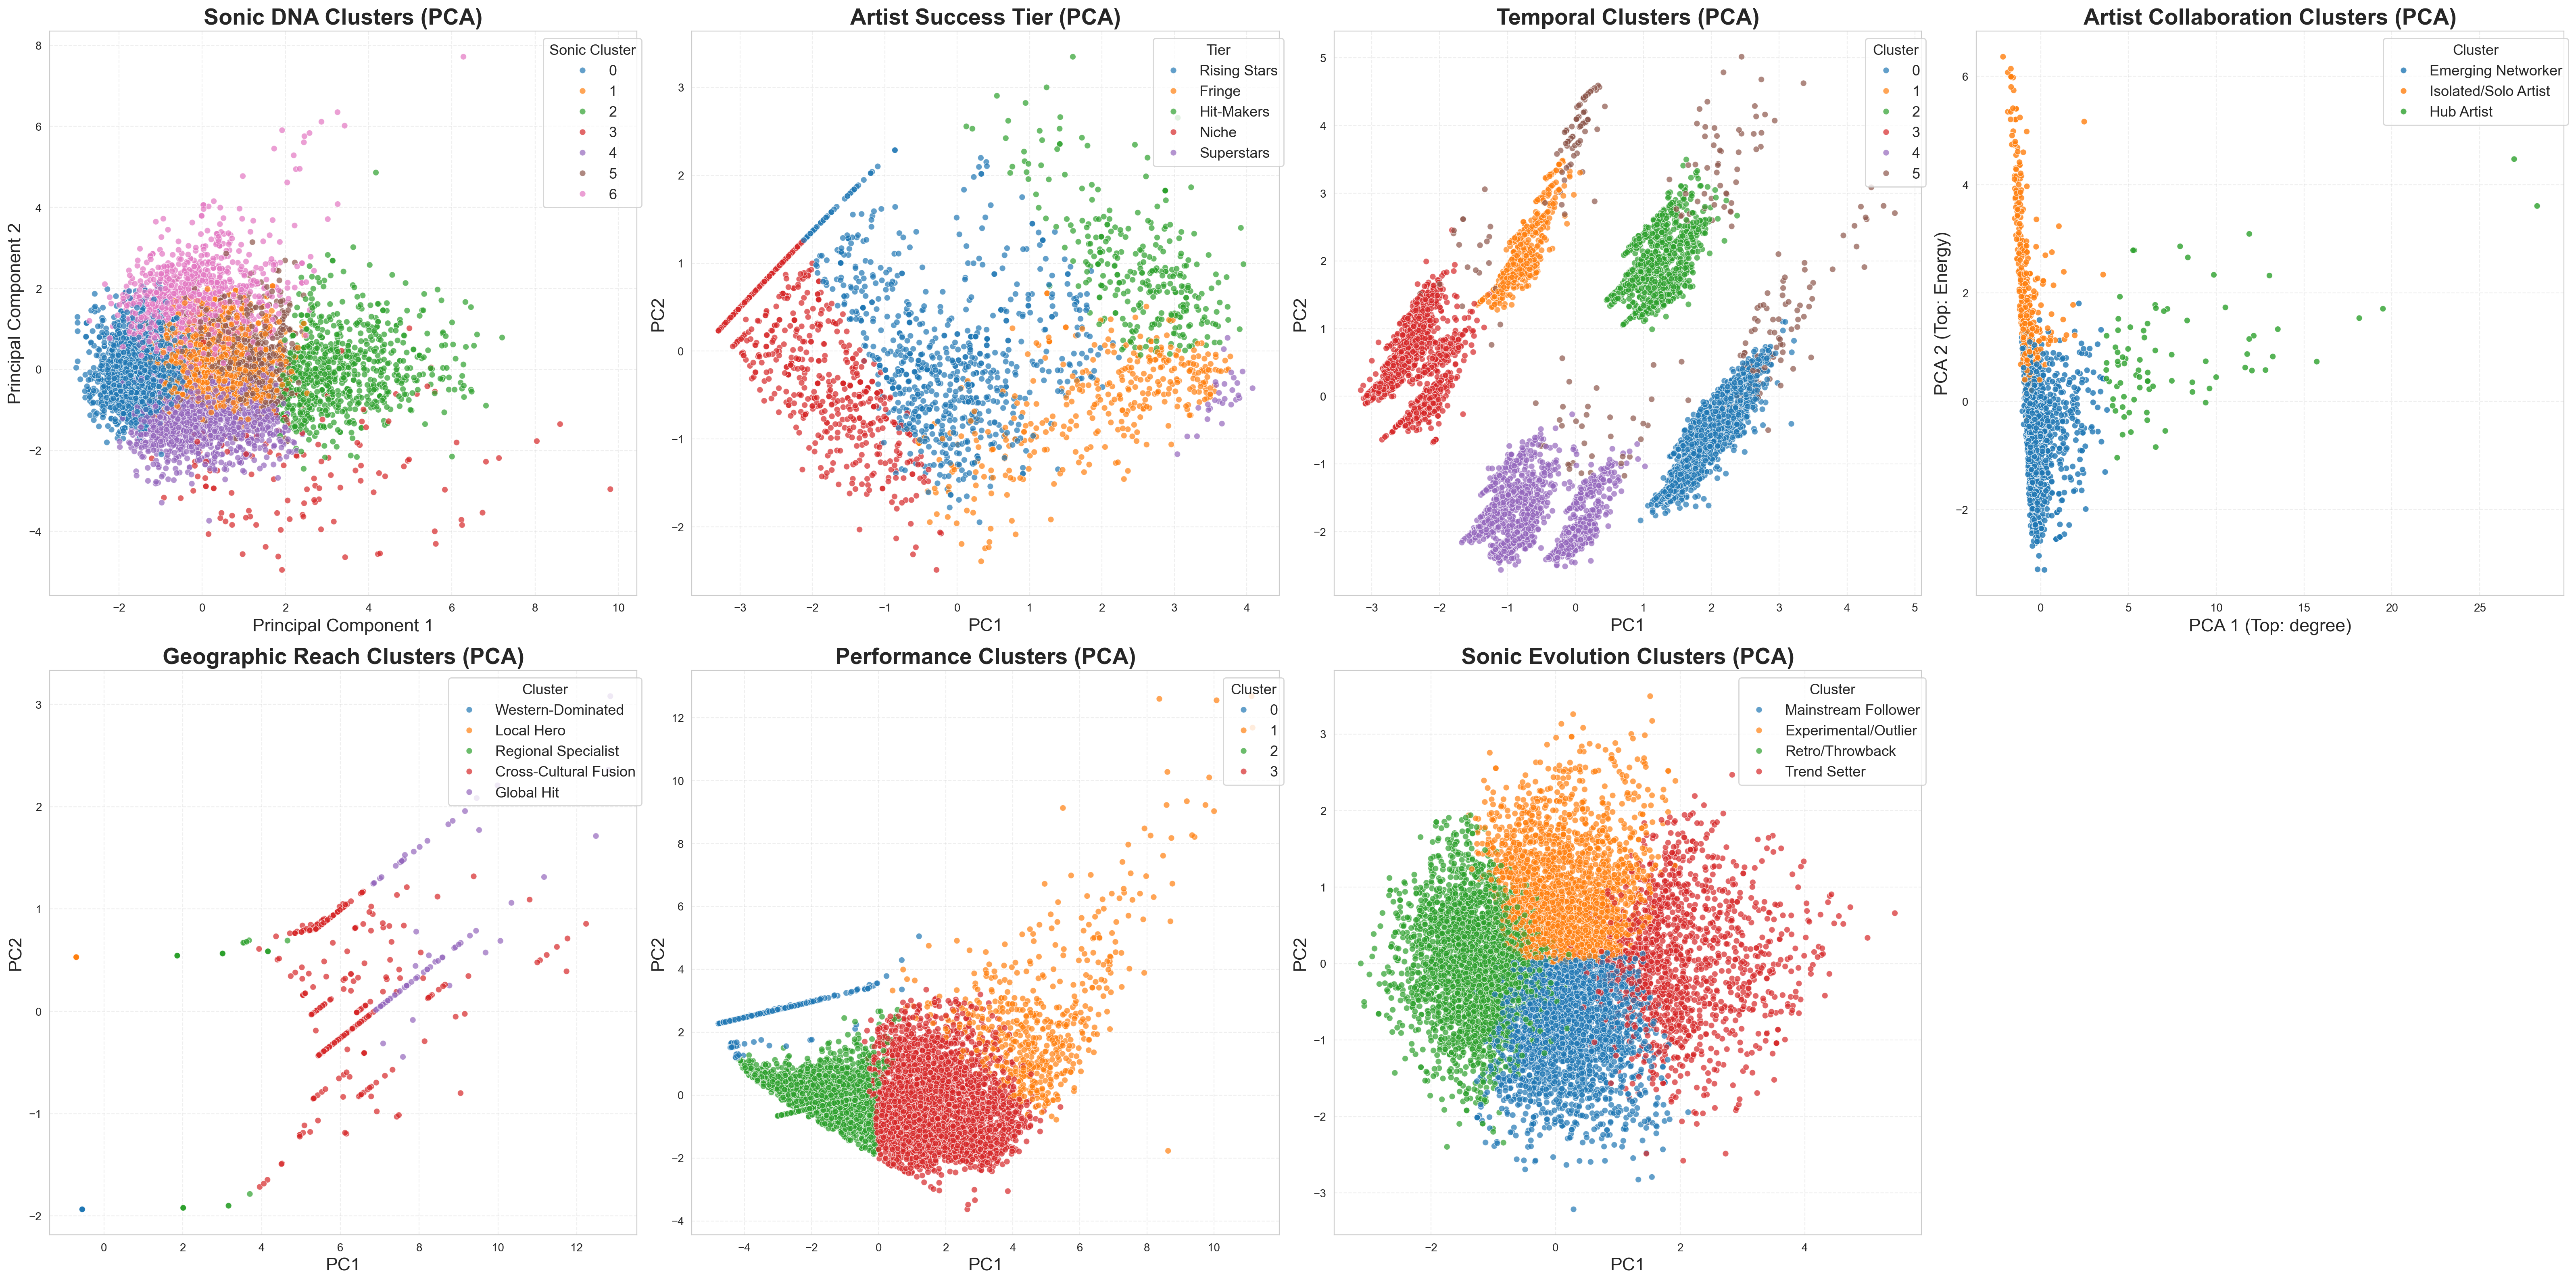
\includegraphics[width=1\textwidth]{figs/combined_pca_cluster_plots_final.png}
  \caption{Comparison of all clustering results from the study.}
  \label{fig:combined_clustering}
\end{figure}
The multi-dimensional analysis identified distinct archetypes across the music landscape: \textbf{Sonic Profiles} (e.g., High-Energy Pop), \textbf{Artist Success Tiers} (Superstars to Newcomers), \textbf{Release Patterns} (Time-sensitive), and \textbf{Performance Trajectories} (Viral Hits vs.\ Long-Term Mainstays). The generated meta-features exhibit diverse market behaviors: performance clustering differentiates between short-term virality and longevity, whilst geographic and network analyses capture global reach and collaborative influence, effectively transforming raw metrics into interpretable, high-level signals.

\subsection{Binary classification} 
The Random Forest classifier achieved the highest performance with \textbf{ROC-AUC of 0.690 and accuracy of 0.699}, outperforming Logistic Regression (0.617 ROC-AUC), XGBoost (0.680 ROC-AUC), and Gradient Boosting (0.679 ROC-AUC). For imbalanced datasets, ROC-AUC is the preferred metric as it better reflects discriminative performance across both classes. The initial model using all seven clusters achieved approximately 98\% ROC-AUC, but after removing leaky features that encode chart outcomes, performance decreased to 69\% ROC-AUC.

\subsection{Multiclass classification}
The 3-class formulation significantly outperformed our initial 4-class attempt \cite{berg2022one}, with Gradient Boosting achieving 58.86\% weighted F1-score compared to 53.18\% in the 4-class version. This 5.68 percentage point improvement confirmed that our decision to merge the ambiguous middle categories was indeed correct. Surprisingly, both the optimization strategies failed to improve performance. This suggested that the default parameters were already quite well-optimized for our dataset.While our final 58.86\% F1-score falls 11.14 percentage points short of the 70\% target we had set for ourselves, this does reflect a 25.5 percentage point improvement over random guessing at 33.33\%.

\subsection{Regression}
Across the evaluated regressors, the tuned LightGBM model delivered the strongest predictive accuracy, achieving \textbf{$RMSE$ = 0.308, $MAE$ = 0.186, and $R^2$ = 0.888} in the transformed target space. When converted back to weeks for interpretability, it obtained \textbf{$RMSE$ = 5.35 weeks, $MAE$ = 1.91, and $R^2$ = 0.716}, indicating that the model explains a substantial share of the variability in chart longevity despite the noisy nature of real-world song performance. These values suggest the model is well-calibrated: errors are typically within a few weeks of the true duration, and the high $R^2$ highlights strong generalisation even under temporally ordered evaluation. SHAP analysis[\ref{app:SHAP}] provided insight into which features drove each prediction, decoding the model's behaviour.

\subsection{Ablation Analysis}
The ablation study gives conclusive evidence that multi-cluster meta-features greatly enhance the predictive performance across all modeling tasks.
\vspace{-0.5em}
\begin{enumerate}[itemsep=0.5ex, topsep=0pt, parsep=0pt, partopsep=0pt, leftmargin=*]
    \item \textbf{Quantitative Performance Lift} 
    In the regression task, the "Clusters Only" model achieved an $R^2$ of \textbf{73.07\%}, a significant \textbf{+15.77\% improvement} over the raw audio baseline ($73.07\%$). The Combined model reached an overall peak accuracy of \textbf{88.8\%}, validating the synergistic value of the framework.
    \item \textbf{Dominant Predictors \& Stability} 
    Feature importance analysis identified \texttt{Performance\_Cluster} as the dominant predictor, with importance greater than 0.40, outperforming individual audio features (< 0.10). The original model built using {\textbf{Gradient Boosting}} also had superior stability in 3-Class Classification, reaching a weighted F1-score of \textbf{57.95\%} without requiring synthetic oversampling.
\end{enumerate}
\vspace{-0.6em}
\section{Conclusions}
\vspace{-0.6em}
% The binary classification task successfully distinguished between songs achieving sustained chart success and those that do not. Our analysis revealed that initial models achieved misleadingly high accuracy by relying on features that directly encoded chart outcomes, whereas the final model using only information available at prediction time achieved more modest but realistic performance. This experience demonstrates that sustained chart success depends on factors beyond audio characteristics alone, such as marketing strategy, playlist placements, and artist reputation.
% \\We also conclude that for the multiclass classification, the consistent performance ceiling across multiple optimization attempts including hyperparameter tuning and SMOTE balancing suggests we have captured possibly all the algorithmically predictable components of music success. Having said that, the remaining gap to our 70\% target likely requires external features like social dynamics and marketing spend, that audio-based models simply do not have access to. This work establishes both the promise and fundamental limitations of predicting chart success from streaming platform data alone.
% Also ablation test confirms a significant increase in predictive gains outperforming the baseline. Also \texttt{Performance\_Cluster} is most important feature providing synergistic value beyond individual audio features.

The binary classification task was able to distinguish between songs with long-run chart presence and those that dropped off quickly, though the performance of the final model was more conservative once all features with direct outcome leakage were removed. This provides a clearer picture of what can realistically be predicted from pre-release information alone.
In the multiclass classification setting, even with class rebalancing and hyperparameter optimisation, the models reached a performance plateau. This suggests that the finer-grained distinctions between chart-trajectory categories contain substantial noise that cannot be captured from the available metadata and audio descriptors.\\
For the regression task, the models explained part of the variation in chart duration, but a considerable portion remained unpredictable. This was consistent with the residual structure and with the ablation study, which showed that meta-features, particularly \textbf{performance-based clusters}, contribute meaningfully beyond audio features but still leave much variance unaccounted for.\\
Overall, these results indicate that while machine-learning models can extract useful signals about potential chart success, the predictability ceiling was largely shaped by external factors such as marketing, exposure, and broader cultural dynamics that fall outside the scope of streaming-derived data. The project therefore highlights both the strengths of data-driven prediction and the inherent limitations of modeling a phenomenon influenced by many unobserved variables.
\newpage
% \section*{Citations and References}
% You can manage your bibliography---adding citations and references to other work---through BibTeX.
% Please see \url{https://www.overleaf.com/learn/latex/Bibliography_management_with_bibtex} for guidance.

% We show a minimal example of how to use it here.

% \LaTeX{} \cite{latex2e} is a set of macros built atop \TeX{} \cite{texbook}.

\bibliography{refs.bib}
\bibliographystyle{plain}


\newpage
\appendix
\section*{Appendix A: Clustering and Meta-Data Generation}
\begin{table}[htbp]
\centering
\caption{Summary of Clustering Dimensions and Resulting Labelled Groups}
\begin{tabular}{p{0.3cm} p{2.8cm} p{1.8cm} p{4.5cm} p{4.2cm}}
\toprule
\textbf{No.} & \textbf{Clustering Dimension} & \textbf{Model Used} & \textbf{Features Used} & \textbf{Labelled Clusters / Tiers Produced} \\
\midrule
1 & Audio / Musical Style Clusters & K-Means (K=7) & Danceability, Energy, Valence, Acousticness, Instrumentalness, Speechiness, Loudness & ``High-Energy Dance'', ``Mellow \& Acoustic'', ``Intense/Dark'', ``Rap/Spoken Word'', ``Instrumental/Ambient'', ``Feel-Good Pop'' \\
\addlinespace
2 & Artist Success Tier Clusters & K-Means or Hierarchical (K=5) & Total chart appearances, Average rank, Best rank, Top-50 rate, Collaboration rate, Career length, Recent momentum & ``Superstars'', ``Rising Stars'', ``Established Mid-Tier'', ``One-Hit Wonders'', ``Newcomers'' \\
\addlinespace
3 & Temporal / Era Clusters & K-Means (K=6) & Year and month of first appearance, Chart longevity, Peak timing, Decay pattern & ``Recent Era (2022-2023) - Winter'', ``Spring - Friday Fresh'', ``Viral/Quick Peak - Winter'', ``Recent Era (2022-2023) - Sustained Success'', ``Early Era (2017-2018) - Viral/Quick Peak'', ``Early Era (2017-2018) - Summer'' \\
\addlinespace
4 & Collaboration Network Clusters & K-Means (K=3) & \# Collaborators, Network centrality, Avg. success of collabs, Collab diversity, Solo–collab ratio & ``Emerging Networker'', ``Hub Artist'', ``Isolated/Solo Artist'' \\
\addlinespace
5 & Geographic / Market Clusters & K-Means (K=5) & Nationality count, Continent of origin, Intl. collaboration, Geographic diversity score & ``Global Hit'', ``Regional Specialist'', ``Local Hero'', ``Western-Dominated'', ``Cross-Cultural Fusion''' \\
\addlinespace
6 & Performance Pattern Clusters & K-Means (K=4) & Avg. rank, Rank volatility, Total points, Peak rank, Weeks in Top 50/10, Rank improvement rate & ``Volatile Performer'', ``Lower-Chart Resident'', ``Strong Performer'', ``Mid-Chart Mainstay'' \\
\addlinespace
7 & Audio Evolution Clusters & K-Means (K=4) & All 7 sonic audio features(Danceability, Energy, Loudness, Speechiness, Acousticness, Instrumentalness, Valence) + release year & ``Trend Setters'', ``Mainstream Followers'', ``Retro/Throwbacks'', ``Experimental / Outliers'' \\
\bottomrule
\end{tabular}
\label{tab:clustering_summary}
\end{table}

\section*{Appendix B: Binary Classification}
\label{app:binary}
\subsection*{Problem Formulation}

Binary classification distinguishes between songs achieving sustained chart success (8 or more consecutive weeks in the Top 200) and those that do not. The target distribution reflects realistic chart dynamics: 25.2\% of songs achieved sustained success while 74.8\% did not, creating a moderately imbalanced classification task.
\subsection*{Model Evaluation and Optimization}

We evaluated four classifiers: Logistic Regression (linear baseline), Random Forest, Gradient Boosting, and XGBoost. All models were trained on 13 features comprising 7 raw audio characteristics (Danceability, Energy, Loudness, Speechiness, Acousticness, Instrumentalness, Valence) and 4 cluster meta features (Sonic\_Cluster, Artist\_Tier, Collab\_Cluster\_ID, Continent). Data was split 80 and 20 with stratification on the target variable. Class weighting was applied during training to account for the imbalanced class distribution. Hyperparameter tuning via GridSearchCV was attempted on top performers, but optimization did not improve baseline performance.

\subsection*{Classifier Performance}
\begin{table}[h]
\centering
\caption{Binary Classification: All Classifiers and Performance Metrics}
\label{tab:binary_all_classifiers}
\begin{tabular}{lcccc}
\toprule
\textbf{Classifier} & \textbf{ROC-AUC} & \textbf{Accuracy} & \textbf{Precision} & \textbf{Recall} \\
\midrule
Logistic Regression & 0.617 & 0.570 & 0.69 & 0.57 \\
Gradient Boosting & 0.679 & 0.73 & 0.69 & 0.73 \\
XGBoost & 0.680 & 0.66 & 0.71 & 0.66 \\
Random Forest & 0.690 & 0.699 & 0.72 & 0.70 \\
\bottomrule
\end{tabular}
\end{table}

Random Forest achieved the highest ROC-AUC of 0.690 and 69.9\% accuracy, outperforming the linear baseline (0.617 ROC-AUC). The 7.3 percentage point gap between Logistic Regression and Random Forest indicates that non-linear interactions between features are essential for distinguishing sustained from non-sustained performers.


\subsection*{ROC Curves Across All Classifiers}

\begin{figure}[h]
\centering
\includesvg[width=0.85\textwidth]{figs/roc_curve_comparison.svg}
\caption{ROC Curves for All Binary Classifiers. Random Forest achieved the highest area under the curve (0.690), outperforming Logistic Regression (0.617), Gradient Boosting (0.679), and XGBoost (0.680).}
\label{fig:roc_curves}
\end{figure}

\subsection*{Feature Importance and Per Class Performance}

\begin{figure}[h]
\centering
\includesvg[width=0.85\textwidth]{figs/feature_importance.svg}
\caption{Random Forest Feature Importance. Loudness (14.0\%), Danceability (12.4\%), and Speechiness (12.9\%) were the top predictors. Continent (11.6\%) ranked fourth. Cluster meta features contributed less: Artist\_Tier (6.8\%), Sonic\_Cluster (3.5\%), Collab\_Cluster\_ID (2.1\%).}
\label{fig:feature_importance}
\end{figure}
Audio characteristics dominated feature importance, collectively accounting for over 62\% of predictive power. Loudness emerged as the strongest single predictor, suggesting that production quality substantially influences chart longevity. Geographic reach (Continent) ranked fourth, indicating that regional market dynamics matter significantly. Collaboration network position (Collab\_Cluster\_ID) and sonic clustering (Sonic\_Cluster) contributed minimally, suggesting that a song's success depends more on intrinsic audio qualities than on positioning within established production archetypes.
\begin{table}[h]
\centering
\caption{Random Forest Confusion Matrix and Per Class Metrics (n=1,833)}
\label{tab:confusion_matrix}
\begin{tabular}{lcc}
\toprule
& \textbf{Predicted Non sustained} & \textbf{Predicted Sustained} \\
\midrule
\textbf{Actual Non sustained (1,372)} & 1,042 & 330 \\
\textbf{Actual Sustained (461)} & 221 & 240 \\
\bottomrule
\end{tabular}
\end{table}

The model achieved 76\% accuracy on the non sustained class but only 42\% precision on sustained songs, generating 330 false positives. The sustained class reached 52\% recall, indicating the model identifies just over half of genuinely successful songs. This asymmetry reflects a fundamental challenge in predicting early success: songs with similar audio profiles and artist characteristics can diverge sharply in chart performance based on external factors (marketing, playlist placement, social dynamics) not available in the feature space.

\begin{figure}[h]
\centering
\includesvg[width=0.85\textwidth]{figs/precision_recall_curve.svg}
\caption{Precision-Recall Curve for Random Forest (AUC = 0.403). The sharp initial drop illustrates the challenge of predicting the minority sustained class without excessive false positives.}
\label{fig:precision_recall}
\end{figure}

\subsection*{Error Patterns and Model Limitations}

The 330 false positives represent the primary failure mode: non sustained songs incorrectly predicted as sustained. This misclassification reflects the difficulty in distinguishing genuine long term success from early chart momentum using audio features alone. Conversely, the 221 false negatives indicate that some sustained performers lack audio characteristics typical of successful songs, suggesting that artist reputation, marketing, or playlist placement compensate for less conventional audio profiles.

\subsection*{Key Findings}

Random Forest's superiority over linear and other ensemble methods confirms that chart success involves non linear interactions between multiple feature types. The 330 false positives demonstrate that audio characteristics alone cannot reliably predict sustained success; external factors determine outcomes. Production quality (Loudness) and vocal characteristics (Danceability, Speechiness) matter more than conformity to sonic archetypes. The precision recall imbalance reveals that high confidence prediction of sustained success requires information unavailable at release time.
\section*{Appendix C: Multiclass Classification}

\subsection*{Problem Formulation and Feature Engineering}
We developed a multiclass classifier to predict a song's success across 3 categories: Flop (under 2 weeks on chart), Moderate Hit (2 to 20 weeks), and Long-Term Hit (20+ weeks). This formulation emerged after our initial experiments with 4-class categorization, by separating Moderate Hit into Brief Hit and Sustained Success, which yielded only 53.18\% weighted F1-score, due to overlapping feature distributions in the middle categories. Merging these into a unified Moderate Hit category improved performance to 58.86\%, a 5.68 percentage point gain, establishing more distinct decision boundaries.

\subsection*{Model Evaluation and Optimization Experiments}
We evaluated 5 baseline algorithms representing a variety of learning methodologies, out of which, Gradient Boosting achieved the highest performance at 58.86\% weighted F1-score, outperforming the alternatives by 0.4 to 8.2 percentage points (Figure~\ref{fig:app_models}).

Following the baseline models' analysis, we attempted 2 optimization strategies that surprisingly yielded negative results. Firstly, the hyperparameter tuning via GridSearchCV explored 108 configurations per model using a 3-fold cross-validation, varying parameters including n\_estimators (100, 200, 300), max\_depth (3, 5, 7 for GB; 5, 10, 15 for XGB), learning\_rate (0.01, 0.1, 0.2), and regularization settings. Instead of improving the performance, tuning surpsisingly degraded Gradient Boosting by 1.05 percentage points (58.86\% to 57.82\%), and XGBoost by 0.17 points (58.46\% to 58.29\%). This implies that sklearn's default configurations are already well-calibrated for problems of this scale.

Secondly, we tried SMOTE oversampling to address the 2.11:1 class imbalance ratio (expanding training data from 7,328 to 9,015 samples with perfect class balance), which showed alarmingly negligible impact. Gradient Boosting with SMOTE declined 0.66 percentage points, while XGBoost improved marginally by 0.24 points. These negative optimization results indicate that neither hyperparameters being suboptimal nor any class imbalance constitute the primary performance bottlenecks. The consistent $\sim$59\% F1 ceiling across strategies suggests limitations in the fundamental feature space.

\begin{figure}[t]
\centering
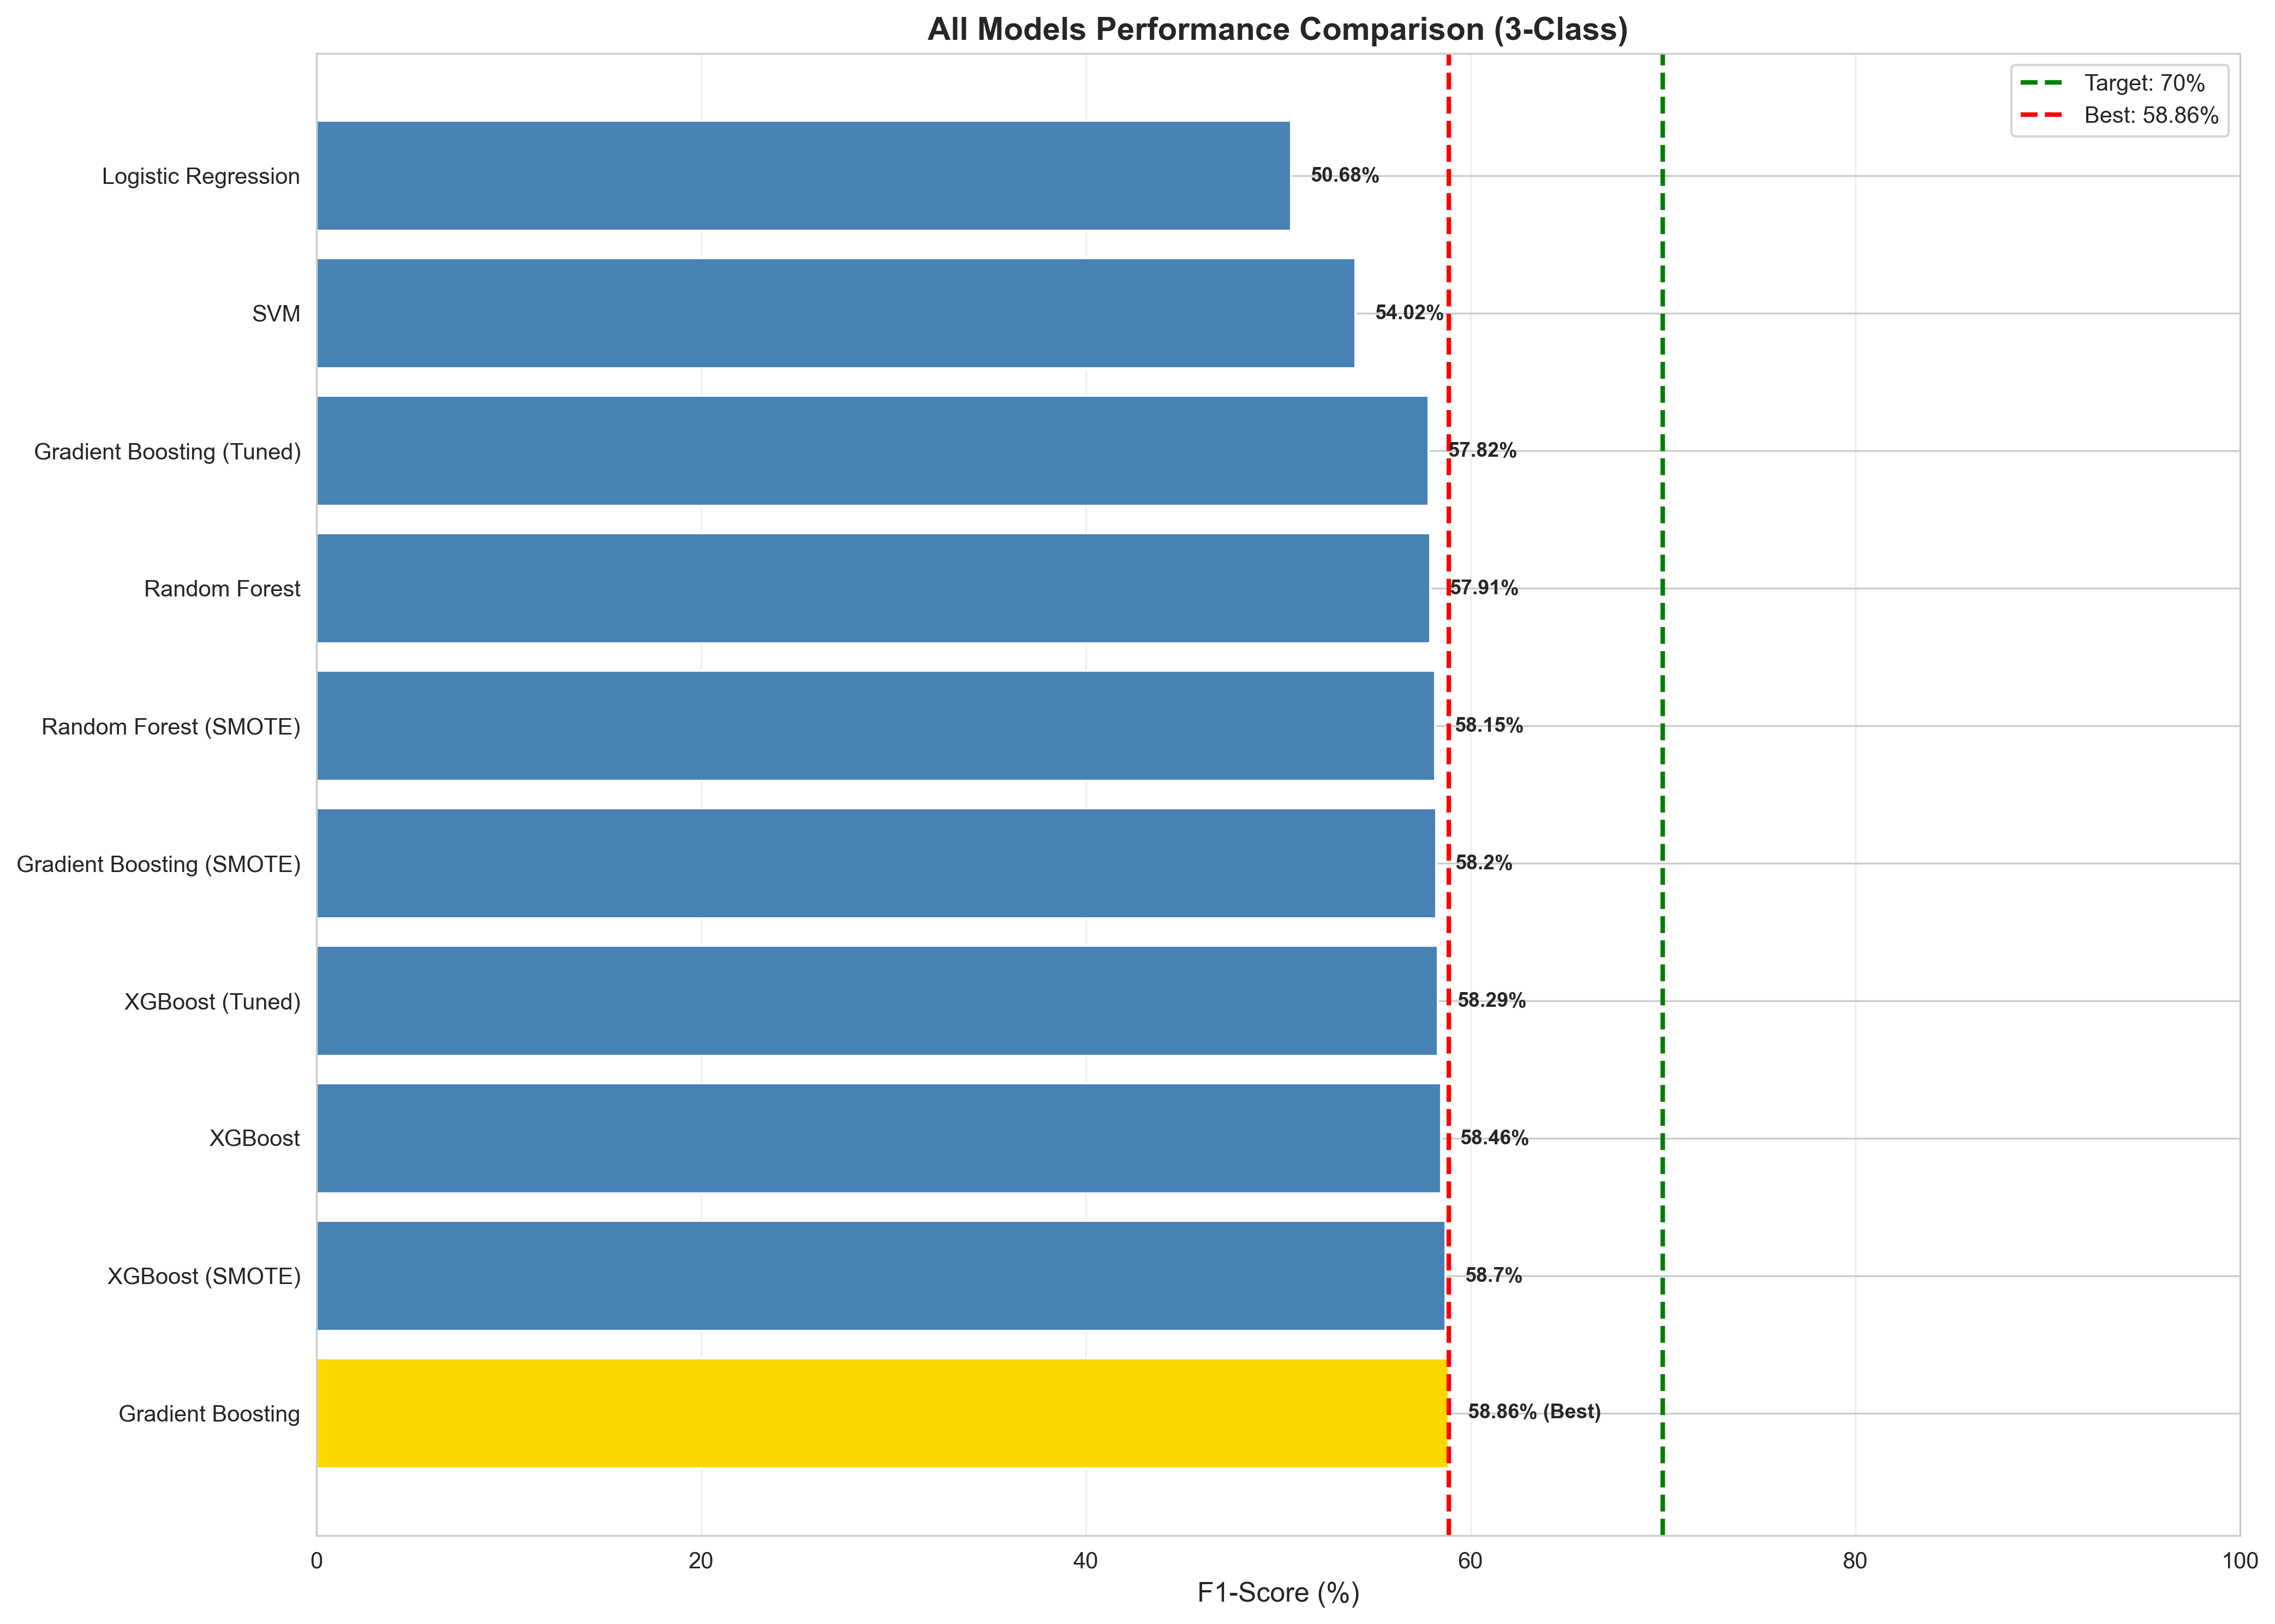
\includegraphics[width=0.58\textwidth]{figs/all_models_comparison_final_3class.png}
\caption{Weighted F1-scores across all the evaluated configurations. The tight clustering of tree-based methods between 57-59\% indicates a robust performance ceiling with current features.}
\label{fig:app_models}
\end{figure}

\subsection*{Error Pattern Analysis}
Confusion matrix analysis (Figure~\ref{fig:app_confusion}) reveals systematic error patterns providing insight into our model's limitations. The primary failure mode involves misclassifying several Flops as Moderate Hits, as seen in 131 of 357 Flop instances (36.7\%). This confusion shows us somewhat of an expected unpredictable nature of early chart failure, which often results from external factors which are beyond our feature space, including marketing campaign timing, competitive releases in the same week, playlist placement delays, or just pure bad luck in terms of social media virality.

We did observe that the Long-Term Hits exhibited the strongest prediction accuracy with 68.92\% recall and minimal confusion with Flops (only 24 misclassifications, amounting to 3.3\%). Songs that are achieving sustained chart presence for 20+ weeks possess distinctive and relatively easily learnable patterns, which are captured effectively by Performance\_Cluster assignments, and consistent audio characteristics associated with broad audience appeal. However, 225 Long-Term Hits (31.1\%) were misclassified as Moderate Hits, indicating the model's somewhat concerning incapability in distinguishing between very good (15 weeks) and exceptional (25 weeks) performance levels.

Moderate Hits showed bidirectional confusion with both adjacent categories, as 391 misclassified as Long-Term Hits (52.0\%) and 177 as Flops (23.5\%). This high error rate reflects the inherent diversity within this category spanning a wide temporal range (2-20 weeks) that encompasses diverse success, from brief popularity spikes to near-long-term success. The class, in  effect, serves as a catch-all for "middle performance," making consistent prediction challenging.

\begin{figure}[t]
\centering
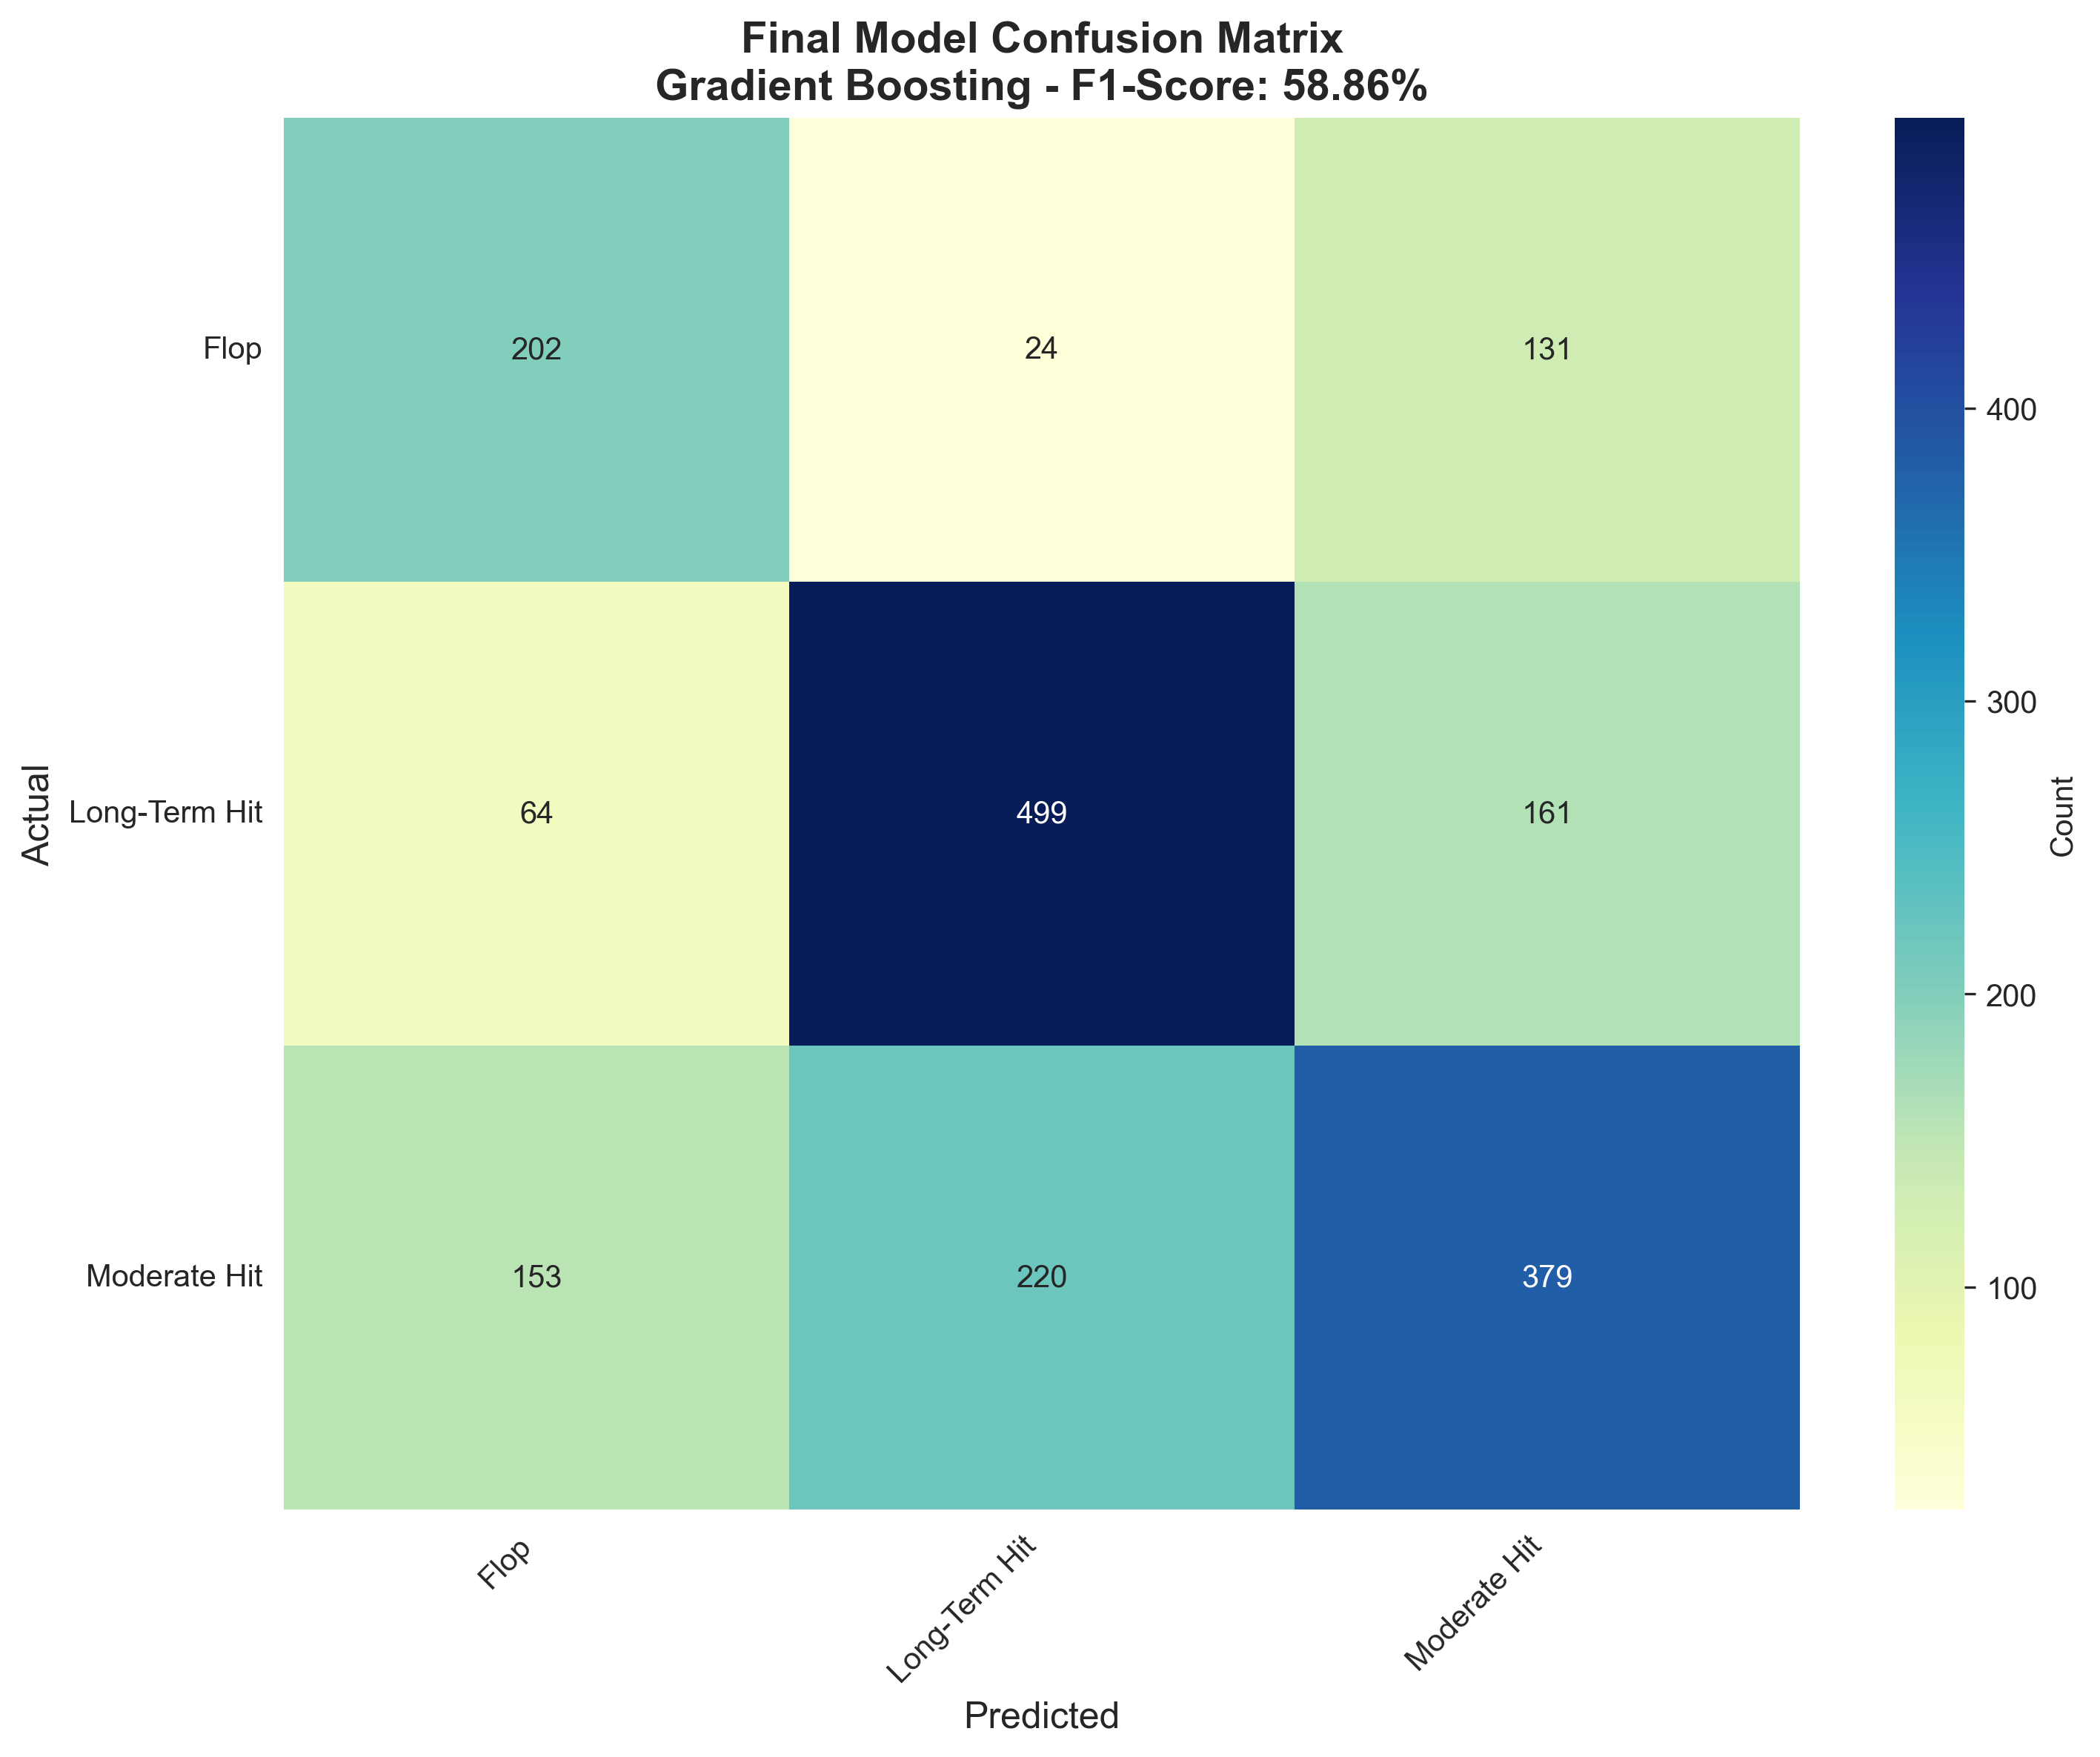
\includegraphics[width=0.48\textwidth]{figs/final_model_confusion_matrix_3class.png}
\caption{Confusion matrix for Gradient Boosting classifier showing predicted vs actual success categories.}
\label{fig:app_confusion}
\end{figure}

\subsection*{Prediction Confidence and Model Calibration}
Our analysis of prediction confidence (Figure~\ref{fig:app_confidence}) reveals meaningful but imperfect model calibration with implications for deployment. For each test prediction, we extracted the maximum probability across the 3 classes as a measure of confidence. The distribution showed a mean of 55.2\% and a median of 53.8\%, indicating substantial amount of uncertainty in many predictions. Only 8.3\% of the predictions exceeded 90\% confidence, while 31.7\% were between 80-90\%, 42.5\% between 60-80\%, 15.2\% between 40-60\%, and 2.3\% were below 40\%.

Critically, the model exhibits meaningful separation between correct and incorrect predictions. Correct classifications averaged 57.4\% confidence while incorrect ones averaged 51.8\%, a 5.6 percentage point gap. This positive correlation demonstrates that the model possesses some level of awareness of the prediction difficulty, and is more confident when it's correct. Having said that, there is a substantial amount of overlap that exists between the distributions, meaning high confidence does not guarantee correctness nor low confidence guarantee error.

Break down w.r.t. predicted class revealed that Long-Term Hit predictions received highest average confidence at 58.9\%, followed by Moderate Hits at 54.1\%, and Flops at 52.3\%. This ordering agrees with the per-class F1-score ranking, suggesting that the model recognizes when it encounters clear signals of sustained success, but it struggles to confidently distinguish between early failure and moderate performance. The calibration also suggests that the deployment scenarios could benefit from confidence-based filtering, where the predictions below a certain threshold (e.g., 50\% confidence) are flagged for human review, or deferred to ensemble methods combining multiple model predictions, which would make the model even more robust.

\begin{figure}[t]
\centering
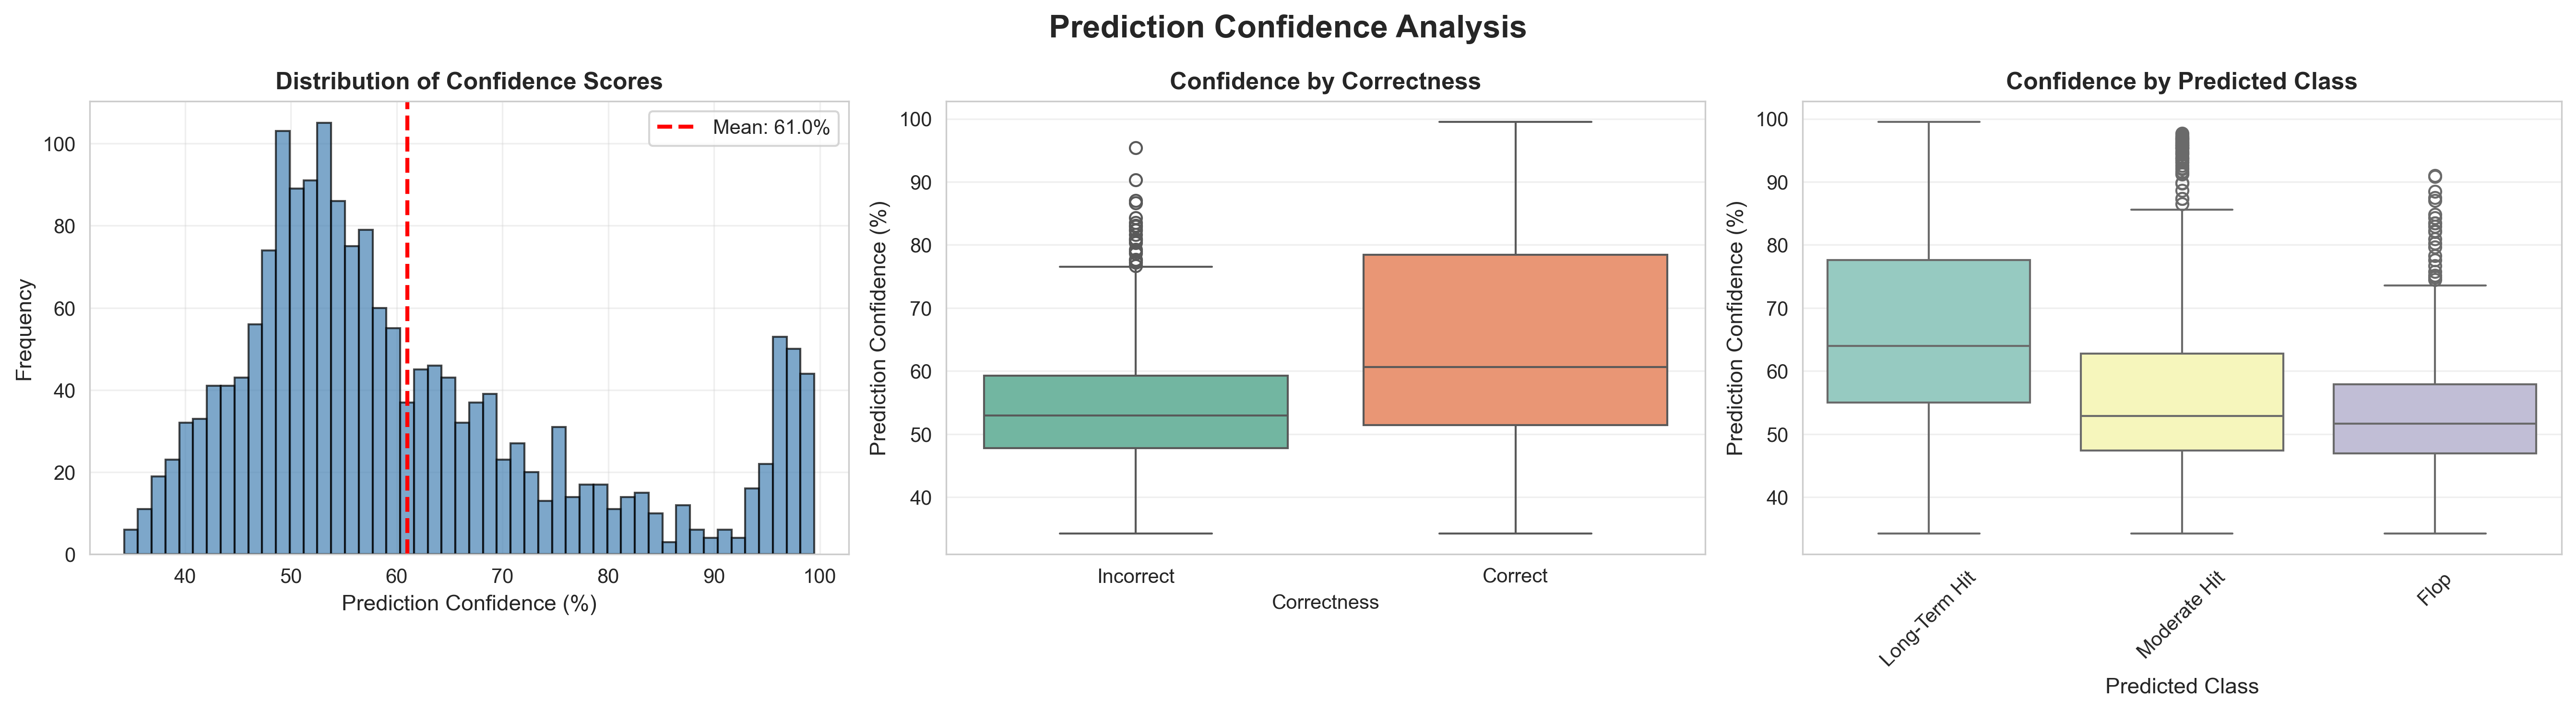
\includegraphics[width=0.98\textwidth]{figs/prediction_confidence_3class.png}
\caption{Prediction confidence analysis across 3 views. \textbf{Left:} Distribution of maximum predicted probability shows mean 55.2\% with substantial uncertainty (only 8.3\% exceed 90\%). \textbf{Center:} Box plots demonstrate correct predictions average 57.4\% confidence vs 51.8\% for incorrect (5.6pp gap), indicating meaningful calibration. \textbf{Right:} Confidence by predicted class shows Long-Term Hits receive highest confidence (58.9\%), consistent with best F1-score. Overall patterns suggest deployment viability with confidence-based filtering for low-certainty cases.}
\label{fig:app_confidence}
\end{figure}

\begin{table}[H]
\centering
\small
\label{tab:app_results}
\vspace{2mm}
\begin{tabular}{@{}lcc@{\hspace{1.8em}}lcc@{}}
\toprule
\textbf{Model Configuration} & \textbf{F1} & \textbf{Acc.} & \textbf{Model Configuration} & \textbf{F1} & \textbf{Acc.} \\
\midrule
Gradient Boosting & \textbf{58.86\%} & 58.92\% & RF (SMOTE) & 58.15\% & 58.97\% \\
XGBoost (SMOTE) & 58.70\% & 58.65\% & Random Forest & 57.91\% & 57.77\% \\
XGBoost & 58.46\% & 58.43\% & Gradient Boost (Tuned) & 57.82\% & 58.15\% \\
XGBoost (Tuned) & 58.29\% & 58.43\% & SVM (RBF) & 54.02\% & 53.68\% \\
Gradient Boost (SMOTE) & 58.20\% & 58.37\% & Logistic Regression & 50.68\% & 50.63\% \\
\bottomrule
\end{tabular}
\caption{Complete model performance comparison showing weighted F1-score and accuracy for all of the evaluated configurations.}
\end{table}

\section*{Appendix D: Regression}
\subsection*{Feature Engineering}
\begin{table}[h]
\centering
\begin{tabular}{l c}
\hline
\textbf{Measure} & \textbf{Skewness} \\
\hline
Raw Target Distribution & 6.11 \\
Log-Transformed Target Distribution & 1.088 \\
\hline
\end{tabular}
\caption{Skewness of the target variable before and after log transformation.}
\end{table}
\begin{figure}[h]
\centering
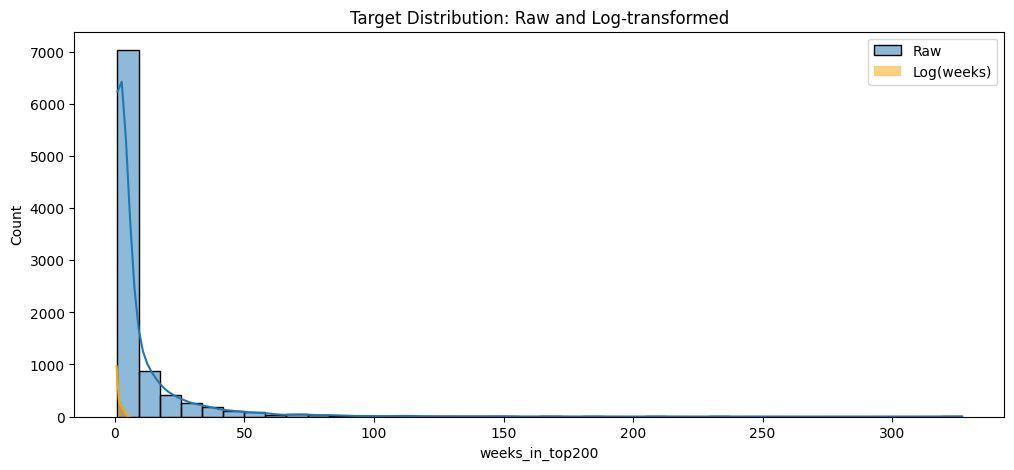
\includegraphics[width=1\textwidth]{figs/regression_target_skew.png}
\caption{Distribution of the target variable (weeks in the Top 200) before and after log transformation. The log transform substantially reduces skewness, producing a more symmetric distribution suitable for regression modeling.}
\label{fig:regression_skew}
\end{figure}
Because the raw target variable (weeks in the Top 200) was extremely right-skewed, we applied a $log(1 + x)$ transformation to stabilise variance and reduce skewness. This produced a more symmetric distribution, allowing the regression models to learn more effectively and avoid being dominated by a small number of long-running songs.

\subsection*{PCA analysis}
\begin{figure}[h!]
\centering
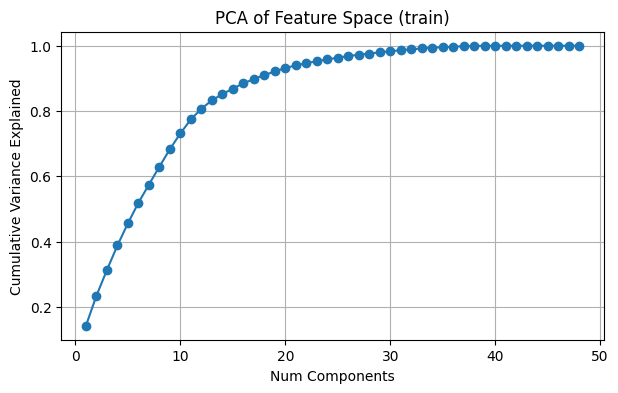
\includegraphics[width=0.7\textwidth]{figs/PCA_regression.png}
\caption{Cumulative variance explained by PCA components in the training dataset.}
\label{fig:regression_pca}
\end{figure}
The PCA curve in Figure \ref{fig:regression_pca}confirms that the feature space is highly multi-dimensional, and preserving all features avoids discarding significant variance (information) present in the data. This justifies working with the full set of input features for our downstream models.

\subsection*{Model Evaluation}
\begin{table}[h]
\centering
\caption{Regression model performance in log-space and back-transformed weeks.}
\begin{tabular}{lccc}
\hline
\textbf{Model} & \textbf{RMSE} & \textbf{MAE} & \textbf{R\textsuperscript{2}} \\
\hline
LGBM (log-space)          & 0.308 & 0.186 & 0.888 \\
Random Forest (log-space) & 0.344 & 0.193 & 0.861 \\
\hline
Best Model (LGBM, back-transformed weeks) & 5.347 & 1.906 & 0.716 \\
\hline
\end{tabular}
\end{table}

The LightGBM model was tuned using a TimeSeriesSplit-based grid search, exploring 32 hyperparameter combinations to account for temporal structure in the data. The search consistently converged on a deeper tree configuration (max\_depth=12) with a moderately fast learning rate (0.1), indicating that the model benefited from greater representational capacity. In parallel, a Random Forest with 300 trees and max\_depth=10 was trained as a benchmark. Overall, the tuned LightGBM model outperformed the Random Forest, achieving the best predictive accuracy and becoming the primary model for subsequent evaluation.

\begin{figure}[h]
    \centering
    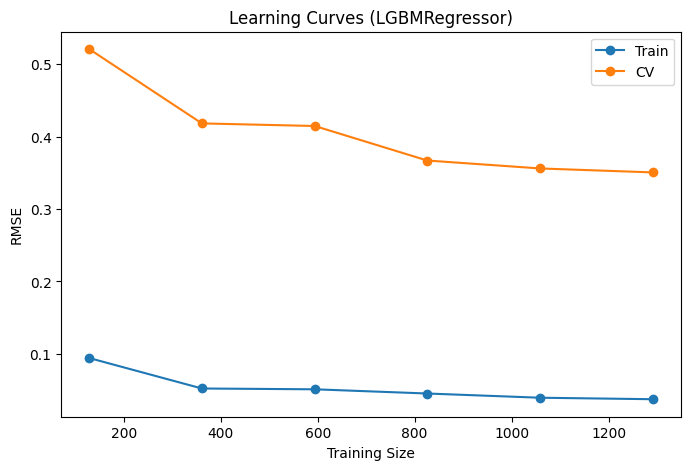
\includegraphics[width=0.55\textwidth]{figs/learning_curves_regression.png}
    \caption{Learning curves for the selected model, showing train and cross-validation RMSE across increasing training sizes.}
    \label{fig:learning-curve-regression}
\end{figure}

\begin{figure}[h]
    \centering
    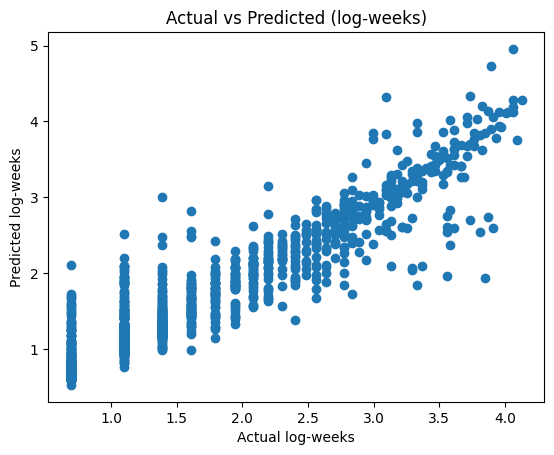
\includegraphics[width=0.55\textwidth]{figs/actual_vs_pred_regression.png}
    \caption{Actual vs predicted values for log-weeks on chart.}
    \label{fig:actual-vs-pred-reg}
\end{figure}
The Figure \ref{fig:actual-vs-pred-reg} shows a positive correlation between actual and predicted log-weeks, indicating that the model predicts chart duration reasonably well. Most points cluster near the diagonal, suggesting good agreement between predictions and true values, though some scatter and outliers remain.

\begin{figure}[h]
    \centering
    \begin{subfigure}[b]{0.32\textwidth}
        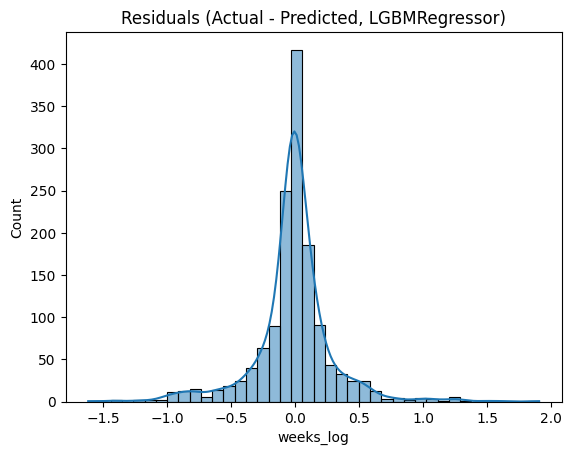
\includegraphics[width=\textwidth]{figs/reg_res_1.png}
        \caption{Histogram of residuals (Actual - Predicted)}
    \end{subfigure}
    \hfill
    \begin{subfigure}[b]{0.32\textwidth}
        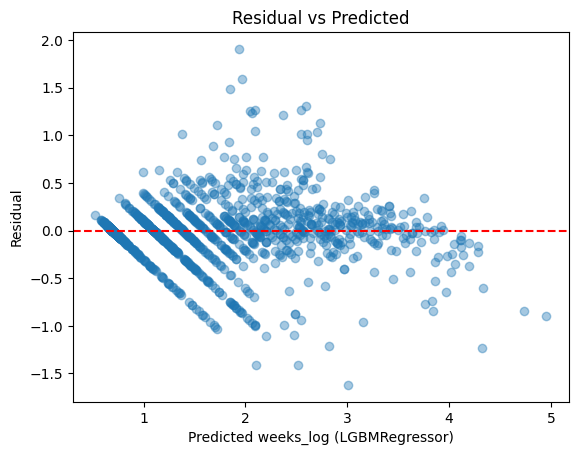
\includegraphics[width=\textwidth]{figs/reg_res_2.png}
        \caption{Residuals vs. Predicted values}
    \end{subfigure}
    \hfill
    \begin{subfigure}[b]{0.32\textwidth}
        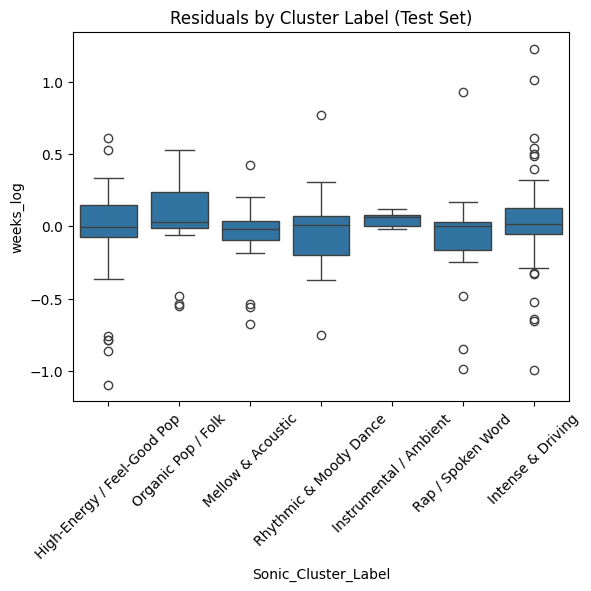
\includegraphics[width=\textwidth]{figs/reg_res_3.png}
        \caption{Residuals by cluster label (test set)}
    \end{subfigure}
    \caption{Residual analysis of the best model (in log space).}
    \label{fig:residual_analysis}
\end{figure}
The residual histogram (a) in Figure\ref{fig:residual_analysis} indicates that the model’s prediction errors are roughly symmetrically distributed and mostly centered near zero, confirming that the model does not consistently over- or under-predict. The scatterplot of residuals vs. predicted values (b) shows no strong heteroscedasticity; however, there is somewhat greater variance for smaller predicted log-week values, suggesting the model may be less precise for songs with shorter chart durations. The boxplot by cluster label (c) reveals that prediction accuracy is broadly similar across distinct musical style clusters, with only minor differences in residual spread or bias among archetypes. Together, these diagnostics suggest robust overall model calibration, reasonably consistent performance across genres, and highlight areas, particularly low predicted values, where further improvements might be targeted.

\subsection*{SHAP Analysis}
\label{app:SHAP}
For each prediction, we conduct a SHAP (SHapley Additive exPlanations) analysis to interpret the most influential features driving model output.
Example (single prediction):
\begin{itemize}[itemsep=0.5ex, topsep=0pt, parsep=0pt, partopsep=0pt, leftmargin=*]
    \item True weeks in top 200: 1
    \item Predicted weeks in top 200: 1
\end{itemize}
Top contributing features to the prediction:
\begin{itemize}[itemsep=0.5ex, topsep=0pt, parsep=0pt, partopsep=0pt, leftmargin=*]
    \item \textbf{Rank slope:} value = -0.82, the strongest negative contributor, reducing the prediction by approximately 0.92 log-weeks.
    \item \textbf{Performance cluster: Volatile Performer:} value = 0.0, slightly lowers the prediction by about 0.14 log-weeks.
    \item \textbf{Points (total):} value = 0.94, increases the prediction by roughly 0.07 log-weeks.
    \item \textbf{Performance cluster: Strong Performer:} value = 0.0, increases the prediction by about 0.06 log-weeks.
    \item \textbf{Performance cluster: Mid-Chart Mainstay:} value = 0.0, raises the prediction by approximately 0.03 log-weeks.
    \item \textbf{Danceability:} value = -0.03, slightly decreases the prediction by about 0.02 log-weeks.
    \item \textbf{Superstar score:} value = -0.52, marginally reduces the prediction by roughly 0.01 log-weeks.
    \item \textbf{Song year:} value = 2.02, increases the prediction by around 0.01 log-weeks.
    \item \textbf{Temporal cluster: Viral/Quick Peak (Winter):} value = 0.0, increases the prediction by about 0.01 log-weeks.
    \item \textbf{Loudness:} value = 0.13, slightly decreases the prediction by roughly 0.01 log-weeks.
\end{itemize}
This SHAP analysis reveals which features most strongly influenced the model’s prediction for a specific song. For this case, the negative rank slope substantially decreased the expected chart duration, indicating a fast drop in rank harms longevity. Not being in the “Volatile Performer” cluster also lowered the outcome, while higher total chart points and various categorical performance labels contributed modest increases. Audio features like danceability and loudness had small effects. Collectively, this breakdown enables a transparent understanding of how the model combines song, artist, and performance traits to produce its prediction for chart duration.

This type of feature-level analysis extends beyond simple prediction, allowing us to diagnose the specific factors that drive a song’s chart success or underperformance. By breaking down the individual contributions of performance metrics, sonic features, and artist attributes, SHAP empowers us to pinpoint what differentiates hits from non-hits, facilitating actionable insights for music creators, analysts, and industry professionals.

\section*{Appendix E: Ablation Study Analysis}
\label{app:ablation}

This appendix presents the complete experimental data and methodological details that support the
Ablation study findings presented in the main text.

\subsection*{Experimental Design}
To validate the multi-cluster framework, we defined three different feature sets for comparative Analysis:
\begin{itemize}
    \item \textbf{Baseline (Raw Features):} Trained only on the 7 intrinsic audio attributes
(\textt{Danceability}, \textt{Energy}, etc.) with basic metadata. This serves as a control to measure the predictive power of the song's features alone.
    \item \textbf{Cluster-Enhanced:} Includes the single most informative meta-feature
\textt{Performance\_Cluster} to the baseline. This variant isolates the specific predictive "lift" provided by modeling chart trajectory archetypes.
    \item \textbf{Full Model:} Uses the complete set of engineered features; all 7 cluster dimensions, including Sonic, Artist, Temporal, among others, for checking synergistic effects.
\end{itemize}

\subsection*{Comprehensive Performance Metrics}
The detailed performance metrics for all three modeling tasks are shown in Table \ref{tab:ablation_full} . These confirm that a consistent hierarchy of performance where the Full Model outperforms the Baseline across all settings. This validates the robustness of the feature engineering framework.


\begin{table}[h]
\centering
\caption{Full Ablation Study Results across Modeling Tasks}
\label{tab:ablation_full}
\begin{tabular}{lccc}
\toprule
\textbf{Feature Set} & \textbf{Regression ($R^2$)} & \textbf{Binary Class. (F1)} & \textbf{3-Class (F1)} \\
\midrule
Baseline (Raw Audio) & 73.07\% & 63.16\% & 42.57\% \\
Cluster-Enhanced & 34.97\% & 76.92\% & 55.18\% \\
\textbf{Full Model (Combined)} & \textbf{88.84\%} & \textbf{78.38\%} & \textbf{57.95\%} \\
\midrule
\textit{Net Performance Lift} & \textit{+15.77\%} & \textit{+15.22\%} & \textit{+14.38\%} \\
\bottomrule
\end{tabular}
\end{table}

\subsection*{Model Selection and Robustness}
Prior to the final ablation test, we conducted a model selection process comparing Logistic Regression, Random Forest, XGBoost, and Gradient Boosting.
\begin{itemize}
    \item \textbf{Algorithm Choice:} The chosen algorithm with the best result is the classifier \textbf{Gradient Boosting}. stability and F1-scores across all feature sets.
    \item \textbf{Hyperparameter Tuning:} Grid search optimization ($CV=3$) was performed but resulted in a negligible performance decrease ($<1\%$), indicating the default parameters were robust for this feature space.
    \item \textbf{Class Imbalance:} Synthetic Minority Over-sampling (SMOTE) was tested for the classification tasks but yielded no significant improvement ($+0.24\%$ F1 lift for XGBoost, negative for others). This means that the characteristics of the engineered cluster successfully linearized the decision boundary; reducing the model's sensitivity to class imbalance without resorting to artificial sampling
\end{itemize}

\newpage
\section*{Statement of Contribution}

\subsection*{S2876894}
Responsible for two of the clustering dimensions: the Artist Collaboration Network Cluster and the Geographical Cluster, including the full data preparation, feature construction, and clustering methodology. Designed and implemented the regression modeling pipeline, conducted model selection, and performed the SHAP-based interpretability analysis to explain feature contributions. On the writing side, I wrote Sections 2, 5 (including Appendix D), and 7.4, and helped write the abstract and Section 3.


\subsection*{S2844528} 
Implemented the Audio Evolution clustering, merged all code samples, and generated the metadata for all clusters. I performed the binary classification to evaluate song success over an 8-week period. I contributed to the report writing for the sections I worked on, including Section 3 (Clustering) and Section 4.1 (Binary Classification), and also wrote the results and conclusion for the binary classification task. Completed the appendix related to the binary classification.


\subsection*{S2843292} Responsible for generating the Audio/Musical Style Clusters and Artist Success Tier clusters. Implemented Ablation Study for all models implemented in this project and contributed to the co-writing of Abstract, Section 1. Also wrote section 6, section 7.1,7.5 and Appendix E related to Ablation Study and clustering.
\subsection*{S2821285}Responsible for generating the performance and temporal clusters and co-writing Section 3. Then continued to work on the multiclass classification problem statement, along with EDA and PCA wherever relevant, followed by co-writing Section 4, and writing Sections 4.2 and 7.3. Contributed to the conclusion by co-writing section 8, followed by working on and writing the entirety of Appendix C, and, at last, writing this statement of contribution.

\section*{Use of GenAI}
We used AI only as a light text editor to improve clarity in parts of our draft and to obtain clarifications about certain concepts. Any suggestions we received were critically evaluated and then fully rewritten in our own words. All code, analysis, and written content submitted in this report were produced by us and not generated by AI.

\end{document}

%%% Local Variables:
%%% mode: latex
%%% TeX-master: t
%%% End:
